%
% File acl2016.tex
%
%% Based on the style files for ACL-2015, with some improvements
%%  taken from the NAACL-2016 style
%% Based on the style files for ACL-2014, which were, in turn,
%% Based on the style files for ACL-2013, which were, in turn,
%% Based on the style files for ACL-2012, which were, in turn,
%% based on the style files for ACL-2011, which were, in turn, 
%% based on the style files for ACL-2010, which were, in turn, 
%% based on the style files for ACL-IJCNLP-2009, which were, in turn,
%% based on the style files for EACL-2009 and IJCNLP-2008...

%% Based on the style files for EACL 2006 by 
%%e.agirre@ehu.es or Sergi.Balari@uab.es
%% and that of ACL 08 by Joakim Nivre and Noah Smith

\documentclass[11pt]{article}
\usepackage{acl2016}
\usepackage{times}
\usepackage{url}
\usepackage{latexsym}
\usepackage{amsmath}
\usepackage{amssymb}
\usepackage{color,soul}
\usepackage[pdftex]{graphicx}
\usepackage{todonotes}

%\aclfinalcopy % Uncomment this line for the final submission
%\def\aclpaperid{***} %  Enter the acl Paper ID here

%\setlength\titlebox{5cm}
% You can expand the titlebox if you need extra space
% to show all the authors. Please do not make the titlebox
% smaller than 5cm (the original size); we will check this
% in the camera-ready version and ask you to change it back.

\newcommand\BibTeX{B{\sc ib}\TeX}
\newcommand\toin{\todo[inline]}

\title{Local Named Entity Disambiguation for Noisy Web Fragments with Neural Attention-RNNs}

\author{First Author \\
	Affiliation / Address line 1 \\
	Affiliation / Address line 2 \\
	Affiliation / Address line 3 \\
	{\tt email@domain} \\\And
	Second Author \\
	Affiliation / Address line 1 \\
	Affiliation / Address line 2 \\
	Affiliation / Address line 3 \\
	{\tt email@domain} \\}

\date{}

\begin{document}
\maketitle
\begin{abstract}
We address the task of Named Entity Disambiguation (NED) in a web setting. We present WikilinksNED, a large-scale NED dataset of short web-page fragments containing mentions manually linked to Wikipedia by web content authors. In contrast to existing news-based datasets the web data is noisier and less coherent. We propose a model based on Attention-RNNs to capture useful features from short and noisy context. We evaluate our model on both WikilinksNED and a standard, smaller, news-based dataset. We find our model greatly outperforms existing state-of-the-art methods on WikilinksNED while achieving reasonable performance on the smaller dataset. We conclude our model can efficiently model noisy context given sufficient training. We analyze our results and show there is room for further improvement on such data.
\end{abstract}



\section{Introduction}

\toin{General comment about citations -- take whatever bibs you can from the ACL anthology: http://aclweb.org/anthology/

The bibs from Google scholar lack a lot of information.}

Named Entity Disambiguation (NED) is the task of linking mentions of entities in text to a given knowledge base, such as Freebase or Wikipedia. NED is a key component in Entity Linking (EL) systems, focusing on the disambiguation task itself, independently from the tasks of Named Entity Recognition (detecting mention bounds) and Candidate Generation (retrieving the set of potential candidate entities). NED has been recognized as an important component in semantic parsing \cite{berant2013semantic}, as well as other NLP tasks.

NED algorithms can broadly be divided into local and global approaches. Local algorithms disambiguate each mention independently using local context (e.g. the sentence in which the mention appeared), whereas global approaches assume some coherence among mentions within a single document, and try to disambiguate all mentions simultaneously. Global algorithms have significantly outperformed the local approach on standard datasets \cite{guo2014entity,pershina2015personalized,Globerson2016}. However, most of these datasets are based on news corpora and Wikipedia, which are naturally coherent, well-structured, and rich in context. Other domains, such as web page fragments, social media, or questions, lack the sufficient coherence and context for global models to pay off. Take for example this fragment taken from the web:

\begin{quote}
	``I had no choice but to experiment with other indoor games. I was born in Atlantic City so the obvious next choice was \textbf{Monopoly}. I played until I became a successful Captain of Industry.''
\end{quote}

This fragment is considerably less structured and with a more personal tone than news reports. It clearly references the entity \textit{Monopoly\_(Game)}, however expressions such as 'experiment', and 'Industry' can generate a lot of noise when disambiguating \textit{Monopoly\_(Game)} from the much more common entity \textit{Monopoly} (economics term). Some sense of local semantics must be considered in order to separate discriminating signals (e.g. indoor games, played) the noisy ones.

In this work, we investigate the task of NED in a setting where only local and noisy context is available. In particular, we create a dataset of 3.2M short text fragments extracted from web pages, each containing a mention of a named entity. Our dataset contains 18K unique mentions linking to over 100K unique entities. This dataset is significantly larger than previously collected ones such as CoNLL-YAGO \cite{hoffart2011robust}, TAC KBP \cite{ji2010overview} and ACE 2010 \cite{bentivogli2010extending}. We have found that performance of state-of-the-art methods is greatly impaired on this dataset and believe new algorithms that can better model local semantic and syntactic features are required.\todo{Try rephrasing the last sentence in less words, simpler terms, and without ``believe''.}

We propose a novel neural network architecture based on Recurrent Neural Networks (RNNs)\todo{no caps} with an attention mechanism, where the RNN units model textual context as a sequence and the attention mechanism gives importance to contextual signals based on the specific candidate entity being evaluated. Our model differs from non-neural approaches by automatically learning feature representations for entity and context, allowing it to extract features from noisy and unexpected context patterns where it can be hard to manually design useful features. We differ from existing neural-based approaches by accounting for the sequential nature of textual context using RNNs and by devising an attention model that can reduce the impact of noise by assigning weights to different contextual signals based on the specific candidate entity being evaluated.

We also describe a novel method for initializing word and entity embeddings used in our model and demonstrate its importance for model performance and training efficiency. 

\toin{Noam: The next sentence sounds odd...}We demonstrate our model greatly outperforms existing state-of-the-art NED algorithms on the web based dataset, showing that existing state-of-the-art methods are not optimal in such settings, and that RNNs with attention can better model noisy and short context. In addition, we evaluate our algorithm on the CoNLL-YAGO dataset \cite{hoffart2011robust}, a dataset of annotated newswire articles, where it yields reasonable results. However it cannot beat state-of-the-art results since it requires large quantities of training data to properly train the large number of parameters in the model. We conclude that RNNs with attention are well-suited for local disambiguation in real-worlds scenarios where context is noisy and less coherent, but analysis of our results reveals that there is still room for improvement.

\section{Background}

\subsection{Related Work}

Early work on Named Entity Disambiguation, such as \newcite{bunescu2006using} and \newcite{mihalcea2007wikify} have focused on local approaches where a mention is disambiguated using hand-crafted statistical and contextual features. While providing a hard-to-beat baseline \cite{Ratinov2011}, increasing attention was recently given to global approaches, which add a layer of sophistication on top of local approaches by considering the coherency of entities assignment within a document. For example the local component of the GLOW algorithm \cite{Ratinov2011} was exploited as part of the Relational inference system suggested by \newcite{Cheng2013}. Similarly, \newcite{Globerson2016} achieved state-of-the-art results by extending the local-based selective-context model of \newcite{Lazic2015} with an attention-like coherence mechanism.

However, \newcite{hoffart2011robust} have found that in many cases global coherency impose false constraints on the relatedness of entities within a document. They used a coherency test to disregard globally suggested Wikipedia entities, and found around $2/3$ of CoNLL's mentions where solved without engaging the global component. We believe that these observations, which were obtained on well structured news articles and Wikipedia based documents, might be amplified in a noisy, non-coherent textual environment such as web content. We have therefore focused on obtaining a strong local, context-based disambiguation solution.

The first published attempt of using DNNs for NED was by \newcite{He2013}, which used stacked auto-encoders to learn a similarity measure between mention-context structures and entity candidates. Recently the increasing popularity of DNNs has inspired a number of works that used Convolutional Neural Nets (CNN) for learning semantic similarity between context, mention and candidate inputs \cite{sun2015modeling,francis2016capturing}. Neural Embedding techniques have also inspired a number of works that jointly map context and entity to the same embedded space \cite{yamada2016joint,Melamud2014}.

In this paper, we train a Recurrent Neural Network (RNN) model, which unlike CNNs and most methods purely based on embeddings, are naturally adapt to exploit the sequential structure of text. Moreover, \newcite{Lazic2015} have used a probabilistic attention-like model and have shown only few context words have value in disambiguating a mention. We therefor experimented with a neural version of an attention mechanism.

\newcite{chisholm2015entity} experimented with using web-link data from the Wikilinks corpus \cite{singh12:wiki-links} for training a disambiguation algorithm. They have shown that despite the noisy nature of web data, augmenting Wikipedia derived data with web-links can lead to improved performance on standard datasets. We make use of the same Wikilinks corpus, but are interested in web data as a noisy test case in-itself rather then using it for training alone. Moreover, in contrast to Chisholm, we use DNNs to automatically capture useful features from the noisy data.

Commonly used benchmarks for NED systems have mostly focused on news-based corpora. CoNLL-YAGO is a dataset based on Reuters newswire articles that was created by \newcite{hoffart2011robust} by hand-annotating the CoNLL 2003 Named Entity Recognition task dataset with YAGO entities. It contains $1393$ documents split into train, development and test sets. TAC KBP 2010 \cite{ji2010overview} is another, smaller, dataset for NED based on news articles. ACE 2005 corpus is another news based dataset annotated by \newcite{bentivogli2010extending}. \newcite{Ratinov2011} have used a random sample of paragraphs from Wikipedia for evaluation, however they did not make the precise sample they used publicly available. 

Our WikilinksNED dataset is substantially different from currently available datasets since these are all based on high quality content from either news-articles or Wikipedia, while WikilinksNED is a test-case for generally noisier, less coherent and lower quality data. The annotation process in significantly different as well, as our dataset reflects the annotation preferences of real-world website authors and is not annotated by experts, or a high-quality community effort in the case of Wikipedia. It is also significantly larger in size, being almost two orders of magnitude larger then all news-based datasets.

Recently, a number of Tweet based datasets have been composed as well \cite{locke2009named, habib2012unsupervised, cano2014making, fromreide2014crowdsourcing}. These represent a much more extreme case then our dataset in terms of noise, shortness and spelling variations, and are much smaller in size. Due to the unique nature of Tweet data, proposed algorithms tend to be substantially different from algorithms used for other NED tasks.

\section{WikilinksNED Dataset: Entity Mentions in the Web}
\label{sec:w}

We introduce a new large-scale NED dataset based on text fragments from the web. Our dataset is derived from the Wikilinks corpus \cite{singh12:wiki-links}, which was constructed by crawling the web and collecting hyperlinks (mentions) linking to Wikipedia concepts (entities) and their surrounding text (context). Wikilinks contains 40 million mentions covering 3 million entities, collected from over 10 million web pages. 

Wikilinks can be seen as a large-scale, naturally-occurring, crowd-sourced dataset where thousands of human annotators provide ground truths for mentions of interest. This means that the dataset also contains various kinds of noise, including erroneous ground-truth labels, malformed mentions, and incoherent contexts. The contextual noise in particular presents an interesting test-case that supplements existing datasets such as CoNLL-YAGO \cite{hoffart2011robust}, TAC KBP \cite{ji2010overview} and ACE 2010 \cite{bentivogli2010extending}, since these datasets are all sourced from mostly coherent and well-formed text (news and Wikipedia). Wikilinks therefore emphasizes the need to understand the local context, and marginalizes the utility of coherency-based global approaches. 

To get a sense of textual noise and entity-context coherence we have set up a small experiment where we measured the similarity between entities mentioned in WikilinksNED and their surrounding context, and compared the results to CoNLL-YAGO. We used state-of-the-art word and entity embeddings obtained from \newcite{yamada2016joint} and computed cosine similarity between an entity embedding and the mean of context words embeddings. We compared results from all mentions in CoNLL-YAGO to a sample of 10000 web fragments taken from WikilinksNED, using a window of words of size 40 around entity mentions. On CoNLL-YAGO we found the mean similarity to be 0.188 while on WikilinksNED we got 0.163.\toin{Noam: we might need to add STD as the difference is very small(not sure if this is statistically significant)} We believe this result indicates that web fragments in WikilinksNED are indeed less coherent and noisier compared to CoNLL-YAGO documents.

We prepared our dataset from the local-context version of Wikilinks,\footnote{\url{http://www.iesl.cs.umass.edu/data/wiki-links}} and resolved ground-truth links using a Wikipedia dump from April 2016\footnote{\url{https://dumps.wikimedia.org/}}. We used the \emph{page} and \emph{redirect} tables for resolution, and kept the database \emph{pageid} column as a unique identifier for Wikipedia entities. We discarded mentions where the ground-truth could not be resolved (only 3\% of mentions).

We collected all pairs of mention $m$ and entity $e$ appearing in the dataset, and computed the number of times $m$ refers to $e$ ($\#(m,e)$), as well as the conditional probability of $e$ given $m$: $P(e|m)=\#(m,e)/\sum_{e'}\#(m,e')$. Examining these distributions revealed many mentions belong to two extremes -- either they had very little ambiguity, or they appeared in the dataset only a handful of times and referred to different entities only a couple of times each.\todo{Not sure I understand the second case. Example? YOTAM: tried to improve explanation. } We deemed the former to be less interesting for the purpose of NED, and suspected the latter to be noise with high probability. To filter these cases, we kept only mentions for which at least two different entities have 10 mentions each ($\#(m,e) \ge 10$) and consist of at least 10\% of occurrences ($P(e|m) \ge 0.1$). This procedure aggressively filtered our dataset and we were left with $3.2M$ mentions.

Finally, we randomly split the data into train (90\%), validation (10\%), and test (10\%), according to website domains in order to minimize lexical memorization (see \cite{levy2015supervised}).


\section{Algorithm}

\toin{This section should be organized as follows: 4. Overview, 4.1. Model Architecture, 4.2. Training, 4.3. Embedding Initialization. Overview should refer to the diagram, which 4.1. elaborates. 4.1. should include all the formulae, as well as the rationale behind the architecture.}

Our DNN model is a discriminative model which takes a pair of local context and candidate entity, and outputs a likelihood for the candidate entity being correct\todo{Omer, check this again. Is it a factor or a probability?}. Both words and entities are represented using embedding dictionaries and we interpret local context as a window-of-words to the left and right of a mention. The left and right contexts are fed into a duo of Attention-RNN (ARNN) components which process each side and produce a fixed length vector representation. The resulting vectors along with the entity embedding are then fed into a classifier network with two output units that are trained to emit the likelihood of the candidate being a correct or corrupt assignment. 

\subsection{Model Architecture}

\begin{figure}
	\centering
	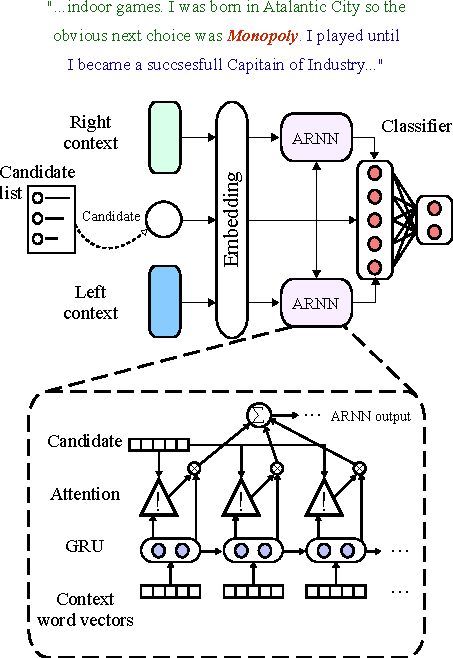
\includegraphics[scale=0.9]{diagrams/model_color_v4.pdf}
	\caption{Architecture of our Neural Network model. A close up of the Attentional RNN component appears in the dashed box.}
	\label{fig:arnn}
\end{figure}	
  
Our architecture has two main component: a duo of ARNN components and a classifier. The classifier network consists of a hidden layer\footnote{300 dimensions with ReLU, and $p=0.5$ dropout.} and an output layer with two output units in a softmax. The output units are trained to emit the likelihood of the candidate being a correct or corrupt assignment by optimizing a cross-entropy loss function. 

The ARNN components each process one side of the context (left and right)\footnote{Right context is fed into the ARNN in reverse order}. The ARNNs are based on a general RNN unit fitted with an attention mechanism, and their mechanics are depicted in Figure \ref{fig:arnn}. 

Equation \ref{eq1} represents the general semantics of an RNN unit. An RNN reads a sequence of vectors $\{v_t\}$ and maintains a hidden state vector $\{h_t\}$. At each step a new hidden state is computed based on the previous hidden state and the next input vector by a function $f$ parametrized by $\Theta_1$. The output at each step is computed from the hidden state using a function $g$ parametrized by $\Theta_2$. This allows the RNN to 'remember' important signals while scanning the context and to recognize signals spanning multiple words.

\begin{equation}
\label{eq1}
\begin{aligned}
& h_t=f_{\Theta_1}(h_{t-1}, v_t) \\
& o_t=g_{\Theta_2}(h_t)
\end{aligned}
\end{equation}

In our implementation we have used a standard GRU unit \cite{cho2014learning}, but any RNN can be a drop-in replacement. We fit the RNN unit with an additional attention mechanism, a mechanism commonly used for state-of-the-art encoder-decoder models where the output of the decoder at time step $t$ is used to decide which parts of the encoder output are important for decoding time step $t+1$ \cite{bahdanau2014neural, xu2015show}. Since our model lacks a decoder, we use the entity embedding as a control signal for the attention mechanism.

Equation \ref{eq2} details the equations governing the attention model.

\begin{equation}
\label{eq2}
\begin{aligned}
& a_t \in \mathbb{R}; a_t=r_{\Theta_3}(o_t, v_{candidate}) \\
& a'_t  = \frac{1}{\sum_{i=1}^{t} \exp\{a_i\}} \exp \{a_t\} \\
& o_{attn}=\sum_{i=1}^{t} a'_t o_t
\end{aligned}
\end{equation}

The main component in equation \ref{eq2} is the function $r$, parametrized by $\Theta_3$, which computes an attention value at each step using $v_{candidate}$, the candidate entity embedding, as a control signal. A softmax function then normalizes the attention values and the final output $o_{attn}$ is computed as a weighted sum of all the output vectors of the RNN. This allows the attention mechanism to decide on the importance of different context parts when examining a specific candidate. We follow \newcite{bahdanau2014neural} and parametrize the attention function $r$ as a single layer NN as shown in equation \ref{eq3} where $A, B$ are the layer weights and $b$ is a bias term.

\begin{equation}
\label{eq3}
r_{\Theta_3}(o_t, v_{candidate}) = Ao_t + Bv_{candidate} + b \\
\end{equation}

\subsection{Training}

We assume our model is only given examples of correct entity assignments during training and therefore automatically generate examples of corrupt assignments. For each context-entity pair $(c,e)$, where $e$ is the correct assignment for $c$, we produce $k$ corrupt examples with the same context $c$ but with a different, corrupt entity $e'$. We have considered two alternatives for corrupt sampling:

\paragraph{Near-Misses:} 
Sampling out of the candidate set of each mention. We have found this to be more effective where the training data reliably reflects the test-set distribution.

\paragraph{All-Entity:} 
Sampling from the entire dictionary of entities. Better suited to cases where the training data or candidate generation does not reflect the test-set well. Has an added benefit of allowing us to utilize unambiguous training examples where only a single candidate is found.

In our evaluation we specify exactly which approach was used for each experiment and provide an empirical comparison of the two approaches.

We sample corrupt examples uniformly in both cases. This matches the distribution of positive examples to the prior probability of the entities for All-Entity sampling and the conditional prior for Near-Misses -- In effect biasing the network towards more popular entities. We note that preliminary experiments revealed that corrupt-sampling according to the distribution of entities in the dataset, rather then uniform sampling (as is done by Mikolov at el. \shortcite{mikolov2013distributed}) produces an interesting entity-context similarity measure, however it does not perform well in our settings due to the lack of biasing toward popular entities.

Model optimization was carried out using standard backpropagation and an AdaGrad optimizer \cite{duchi2011adaptive}. We allowed the error to propagate through all parts of the network and fine tune all trainable parameters, including the word and entity embeddings themselves. We found the performance of our model substantially improves for the first few epochs and then continues to slowly converge with marginal gains, and therefore trained all models for $8$ epochs with $k=5$ for corrupt example generation. 

\subsection{Embedding Initialization}

\begin{table*}[t]
	\begin{center}
		\begin{tabular}{|c| c | c | }
			\hline \multicolumn{3}{|c|}{Wikilinks Test-Set Evaluation} \\
			\hline \bf Model               & \bf Sampled Test Set (10K)  & \bf Full Test Set (300K)  \\
			Baseline (MPS)                 & $60$   & $59.6$ \\
			Cheng et al.                   & $50.7$ & - \\
			Yamada at el.                  & $67.6$ & $66.9$ \\
			\hline
			Our Attention-RNN              & $73.2$ & $73$ \\
			Our RNN, w/o Attention         & $??$   & $??$ \\
			\hline
		\end{tabular}
	\end{center}
	\caption{\label{tab:wikilink} Evaluation on Web-Fragment data (Wikilinks)}
\end{table*}

Training our model implicitly embeds the vocabulary of words and collection of entities in a common space. However, we find that explicitly initializing these embeddings with vectors pre-trained over a large collection of unlabeled data significantly improved both performance and training speed (see Section \ref{experiments}\todo{Refer to the exact subsection where you discuss this result}). To this end, we implemented an SGNS-based approach \cite{mikolov2013distributed} that simultaneously trains both word and entity vectors.

We used \texttt{word2vecf}\footnote{\url{http://bitbucket.org/yoavgo/word2vecf}} \cite{levy2014dependency}, which allows one to train word and context embeddings using arbitrary definitions of "word" and "context" by providing a dataset of word-context pairs $(w,c)$, rather than a textual corpus. In our usage, we define a context as an entity $e$. To compile a dataset of $(w,e)$ pairs, we consider every word $w$ that appeared in the Wikipedia article describing entity $e$. We limit our vocabularies to words that appeared at least 20 times in the corpus and entities that contain at least 20 words in their articles. We ran the process for 10 epochs and produced vectors of 300 dimensions; other hyperparameters were set to their defaults.

\newcite{levy2014neural} showed that SGNS implicitly factorizes the word-context PMI matrix. Our approach is doing the same for the word-entity PMI matrix, which is highly related to the word-entity TFIDF matrix used in Explicit Semantic Analysis \cite{gabrilovich2007computing}.

\section{Evaluation}
\label{experiments}

In this section, we describe our experimental setup and compare our model to the state of the art on two datasets: our new WikilinksNED dataset, as well as the commonly-used CoNLL-YAGO dataset \cite{hoffart2011robust}. We also examine the effect of different corrupt example generation schemes, and of initializing our model with pre-trained word and entity embeddings.

In all experiments, our model was trained with fixed-size left and right contexts (20 words in each direction). We used a special padding symbol when the actual context was shorter than the window. Further, we filtered stopwords using NLTK's stop-word list prior to selecting the window in order to focus on more informative words.

%We experiment with our model both as a standalone model and as a feature along with shallow statistical and string based features. For the second case, we used a setting similar to Yamada et al. \shortcite{yamada2016joint} where a Gradient Boosted Regression Tree was fitted with our models prediction score as a feature along with $7$ other statistical and string based features. The statistical features are prior probability $P(e)$ and conditional probability $P(e|m)$ as described above, along with a feature counting the number of candidates generated for the mention and a feature giving the maximum conditional probability of the entity for all mentions in the document. For string similarity features we used the edit distance between the mention and the entity title in Wikipedia, a feature indicating weather the mention is a prefix or postfix of the entity Wikipedia title and a feature indicating weather the Wikipedia entity title is a prefix or postfix of the mention. Following Yamada we used sklearn's GradientBoostingClassifier implementation \cite{pedregosa2011scikit} with a deviance loss and set the learning rate, number of estimator and maximum depth of a tree to $0.02$, $10000$ and $4$, respectively. 

\subsection{WikilinksNED}

\paragraph{Training} we use Near-Misses corrupt-sampling which was found to perform well due to a large training data that represents the test-data well.

\paragraph{Candidate Generation}
To isolate the effect of candidate generation algorithms, we used the following simple method for all systems: given a mention $m$, consider all candidate entities $e$ that appeared as the ground-truth entity for $m$ at least once in the training corpus. This simple method yields $97\%$ ground-truth recall on the test set.

\paragraph{Baselines}
Since we are the first to evaluate NED algorithms on WikilinksNED, we ran a selection of existing local NED systems and compared their performance to our algorithm's. \textbf{Yamada et al.} \shortcite{Yamada2016} created a state-of-the-art NED system that models entity-context similarity with word and entity embeddings trained using the skip-gram model. We obtained the original embeddings from the authors, and trained the statistical features and ranking model on the WikilinksNED training set. Our configuration of Yamada et al.'s model used only their local features.

\textbf{Cheng et al.} \shortcite{Cheng2013} have made their global NED system publicly available\footnote{\url{https://cogcomp.cs.illinois.edu/page/software\_view/Wikifier}}. This algorithm uses GLOW \cite{Ratinov2011} for local disambiguation. We compare our results to the ranking step of the algorithm, without the global component. Due to the long running time of this system, we only evaluated their method on the smaller test set, which contains 10,000 randomly sampled instances from the full 320,000-example test set.

Finally, we include the \textbf{Most Probable Sense (MPS)} baseline, which selects the entity that was seen most with the given mention during training.

\paragraph{Results}
We used standard micro P@1 accuracy for evaluation on WikilinksNED. Experimental results are reported in Table \ref{tab:wikilink}. Our algorithm significantly outperforms Yamada at el. on this data by over 5 points. This result indicates that the skip-gram model used by Yamada at el. which averages the embedding vectors of all context words is non-optimal compared to our more sophisticated context modeling on this dataset. Our method outperforms the Baseline as well by a very large margin indicating our RNN model is indeed able to capture meaningful contextual features despite the noisy and short context. 

When running Cheng at el \shortcite{Cheng2013} we have used a pre-trained model supplied by Cheng at el which, similarly to the setting used for evaluating the GLOW algorithm by Ratinov at el \cite{ratinov2011glow}, was not directly trained on our training set. This has resulted in poor performance, emphasizing the greater importance of training a model directly on the training set compared to existing datasets based on news corpora and annotated by experts.

We find that the attention mechanism significantly improves results by attending to the most discriminative parts of the context given a specific candidate mention.

\subsection{CoNLL-YAGO}
\label{experiments-conll}

\paragraph{Training}
CoNLL-YAGO has a training set with $18505$ non-NIL mentions, which preliminary experiments showed is not sufficient to train our model on. We therefore resorted to a more complex training method. We first trained our model on a large corpus of Wikipedia derived data, and fine-tuned on CoNLL-YAGO training set. We then used the model in a similar setting to \newcite{yamada2016joint} where a GBRT was trained with our model as a feature along with the statistical and string based features defined by Yamada. 

To derive the Wikipedia training corpus we have extracted all cross-reference links from Wikipedia along with their context, resulting in over $80$ million training examples. We set $k=5$ for corrupt example generation and trained for $1$ epoch with All-Entity corrupt-sampling. The resulting model was then fine-tuned on CoNLL-YAGO training set, where corrupt examples were produced by considering all possible candidates for each mention.

\paragraph{Candidate Generation}
For comparability with existing methods we used two publicly available candidates datasets:
\begin{itemize}
	\item PPRforNED - Pershina at el. \shortcite{Pershina2015}
	\item YAGO - Hoffart at el. \shortcite{hoffart2011robust}
\end{itemize}

\paragraph{Baselines}
As a baseline we took the standard Most Probable Sense (MPS) prediction, which corresponds to the $\arg\max_{e\in{{E}}}{P(e|m)}$, where $E$ is the group of all candidate entities.
We also compare to the following papers - Francis-Landau et al. \shortcite{francis2016capturing},  Yamada at el. \shortcite{yamada2016joint}, and Chisholm et al. \shortcite{Chisholm2015}, as they are all strong local approaches and a good source for comparison.
%He et al. \shortcite{He2013}, Hoffart et al. \shortcite{hoffart2011robust} - YOTAM: I removed these as they are non-local - Make sure again!!%


\paragraph{Results}
The micro and macro P@1 scores on CoNLL-YAGO test-b are displayed in table \ref{tab:conll}. On this dataset our model achieves reasonable results, however it cannot beat state-of-the-art results since it requires large quantities of training data to properly train the large number of parameters in the model. Further, the relative cleanliness of the data allows existing approaches to perform very well and marginalizes the effect of utilizing a deep and powerful neural model.

\begin{table}[h]
	\begin{center}
		\begin{tabular}{|p{3.5cm}| p{1.5cm} p{1.5cm}|}
			\hline \multicolumn{3}{|c|}{CoNLL-YAGO test-b (Local methods)} \\
			\hline Model & Micro P@1 & Macro P@1 \\ 
			\hline \multicolumn{3}{|c|}{PPRforNED} \\
			\hline Our ARNN + GBRT    & $87.3$  & $88.6$ \\
			Yamada et al. local               & $90.9$  & $92.4$ \\
			\hline \multicolumn{3}{|c|}{Yago} \\
			\hline Our ARNN + GBRT    & $83.3$  & $86.3$ \\
			Yamada et al. local               & $87.2$  & $89.6$ \\
			Francis-Landau et al.             & $85.5$  & - \\
			Chisholm et al. local             & $86.1$  & - \\
			\hline
		\end{tabular}
	\end{center}
	\caption{\label{tab:conll} Evaluation on CoNLL-YAGO.}
\end{table}

\subsection{Effects of initialized embeddings and corrupt-sampling schemes}

We performed a study of the effects of using pre-initialized embeddings for our model, and of using either All-Entity or Near-Misses corrupt-sampling. The evaluation was done on a $10\%$ sample of the evaluation set of the WikilinksNED corpus and can be seen in Table \ref{tab:c}. We have found that using pre-initialized embeddings gives a much better starting point for training compared to random initialization. This results in faster convergence and a significant performance gain.

Comparison of All-Entity and Near-Misses corrupt-sampling reveals that when using Near-Misses, our model achieves significantly improved performance. We attribute this difference both to the more efficient nature of training with near misses, and to Near-Misses preserving the conditional-prior of entities which is a stronger signal then the prior probability preserved by All-Entity corrupt-sampling.


\begin{table}[h]
		\toin{YOTAM: ** = Missing one more epoch for Near-misses, random init. - tommorow}
	\begin{center}
		\begin{tabular}{|c| p{1.5cm}|}
			\hline \multicolumn{2}{|c|}{Wikilinks Evaluation-Set} \\
			\hline \bf Model & \bf Micro     accuracy  \\ \hline
			All-Entity, with init. & $70$ \\ 
			All-Entity, random init. & $67.1$ \\ 
			Near-misses, with init. & $72.5$ \\ 
			Near-misses, random init. & $67.2**$ \\ 
			\hline
		\end{tabular}
	\end{center}
	\caption{\label{tab:c} Corrupt-sampling and Initialization}
\end{table}

\subsection{Discussion//Conclusions}
We believe these results demonstrate that our ARNN model is better then existing state-of-the-art techniques at modeling noisy context when sufficient amounts of training examples are available. This allows us to greatly outperform state-of-the-art algorithms which are found to be suboptimal in a noisy environment such as web content. 

However the gap between results of all systems tested on both CoNLL-YAGO and WikilinksNED indicates that web mentions are indeed a more challenging test case then news-based corpora. We believe this to be an important and challenging real-world scenario where noise in the form of mis-structured text, incoherent topics and grammatical/spelling mistakes are present. This scenario represents a distinct test-case that lays in between the standard new-based datasets and the much noisier Tweeter data that has been receiving increasing attention lately. We believe recursive neural models are a promising direction for this task, while there is still much room for improvement. 

\subsection{Error analysis}

We randomly sampled and manually analyzed $200$ individual cases of false disambiguations that our neural model generated. This error subset was obtained from a Wikilinks-based validation set that was not used for training. 

Working with crowd-labeled data, we expected some of the mentions to be associated with wrong Wikipedia titles. Accordingly, we found out that $18$\% (36/200) of the error-labeled predictions were not false, where $21$\% of the mistakes originated in wrong labeling of the author and $34$\% were predictions with an equivalent meaning as the correct entity. %For instance, the music software \textit{Abelton} was labeled under the entity \textit{Abelton live}, a specific version of the program, but assigning it the \textit{Abelton} entity should not be considered an error.
Interestingly, in $11.5$\% (23/200) of the error events, the model suggested a more convincing solution than the original author by using specific hints from the context. In this manner, the  mention \textit{'Supreme leader'} , which was contextually associated to the Iranian leader Ali Khamenei, was linked by our model with \textit{'supreme leader of Iran'} while the "correct" tag was the general \textit{'supreme leader'} entity.
From the remaining $164$ error-entries, $15.5$\% were cases where a Wikipedia disambiguation-page was chosen as either the correct or predicted entity ($2.5$\% and $13$\%, respectively). We decided to discount this error type from further analysis, as it is logically equivalent to remain unresolved. Eventually we ended up with $131$ error cases to analyze.

First, we noticed that in $32$\% of the errors (42/131) the model selected an entity that can be understood as a specific ($7$\%) or general ($25$\%) realization of the correct solution. For example, instead of predicting \textit{'Fu Manchu mustache'} for a facial hair related text, the model addressed the mention with the fictional character \textit{'Fu Manchu'}, with whom the beard style originated. We further investigated and saw that in almost half of those cases, either the predicted or the correct web-page contained a non-trivial link to the other page, thus implying a strong correlation between both entities. Overall, we observed this type of co-reference relation in $26$\% of the error cases (35/131). A closer look discovered two prominent types of co-reference errors that occurred repeatedly in the data. The first category was of a film/book/theater type of error ($9$\%), where the actual and the predicted entities were a different display of the same narrative. Even though having a different jargon and producers, those fields share extremely similar content, which may explain why they tend to be frequently confused by the algorithm. The second issue of the model was in differentiating between adjectives that are used to describe properties of a nation. Particularity, mentions such as \textit{'Germanic'}, \textit{'Chinese'} and \textit{'Dutch'} were falsely assigned to entities that describe language instead of people, and vice versa. We observed this type of mistake in $8.4$\% of the errors (12/131).

A further interesting trend was the prediction policy of the model in cases where the entity had low-count. We defined low-count entities as entities which appeared less than 10 times in the data, and hence were probably not seen in the model's training period. We saw that the model followed the MPS in $75$\% of the low-count events. This shows that entity-mention pairs, which are alien to the model, tend to bias its prediction towards the baseline. Further, the amount of generalization error in low-count conditions was also significant ($35.7\%$), as the uncertainty of the prediction was captured by a similar but less specific entity suggestion.

%While going over the errors, we came across several examples where the actual entity was fully contained in the prediction. For instance, gold-senses such as \textit{'ted'} and \textit{'macedonia'} were "falsify confused" with the entities \textit{'ted (conference)'} and \textit{'republic of macedonia'}. In practice, the context of those examples together with their correct urls links to the same source as the models prediction. This type of error was observed in almost $20$\% of the cases. We also saw that in these $20$\% the conditional prior of the predicted entity was larger than the conditional of the correct sense. We believe that this indicates on the generic nature of the model and emphasizes problems in the candidate generation process.

%A further interesting property of the errors was the distance between the false predicted entity and the correct one. This was measured by calculating the cosine similarity between our word-title embeddings. For example, the similarity between \textit{'the fall (gorillaz album)'} and \textit{'the fall (band)'} was calculated as $0.96$. Accordingly, given that music related words, such as 'recorded' and 'albums', were present in the context of the mention, the decision to pick the wrong sense over the right one does not seem completely detached and irrational. In our analysis the average cosine similarity of the mistakes was estimated to be $0.925$, when $0.9$ was the $20$st percentile of the value distribution. Strong associations between candidates are usually expected in a disambiguation framework, since most possible senses are somewhat related. However, given that the embeddings use as a main feature for our model, we believe that the particularly high error similarity shows that even the wrong predicted entities are strongly related to right senses.    \toin{fix and report with Yamadas embeddings} 

%Lastly, we wanted to check how much our model differs from the MPS baseline by visualizing the error distribution of the conditional prior feature. In this way we could quantify the diversity of the model's prediction. The full error distribution is displayed in. We saw that $64$\% of the error predictions were not most frequent entities. the average conditional prior of those non-mps mistakes was $0.197$\% with $0.664$ coefficient of variation.  Moreover, we observed that $25$st percentile of the error was smaller than $0.09$\%. This error analysis reveals that in most of its mistakes our model does not simply captures [continue]
\bibliographystyle{acl2016}
\bibliography{_our_submission,_noam_bib}

\end{document}
